\begin{center}

  \begin{tabular}{rp{16cm}lp{20cm}}%{rl}

  % after \\: \hline or \cline{col1-col2} \cline{col3-col4} ...

  论文地址:& \href{https://openreview.net/pdf?id=i80OPhOCVH2}{https://openreview.net/pdf?id=i80OPhOCVH2} \\
  来源:& ICLR, 2021 \\
  作者:& Uri Alon, Eran Yahav \\

  源码:& \href{https://github.com/tech-srl/bottleneck/}{bottleneck} \\

%  slides:& \href{http://yunshengb.com/wp-content/uploads/2017/03/nips_2018_r2l_workshop_talk.pdf}{{\footnotesize Convolutional Set Matching for Graph Similarity}}\\

  关键词:& \textbf{GNN, Over-Squashing} \\

  写于:& \date{2021-03-28}

  \end{tabular}

\end{center}

该论文\cite{alon2021on}针对GNN中的远距离信息的传播问题提出了一个新的解释。文中讨论的问题是:GNN在聚集/利用远距离结点的信息时存在困难/一个瓶颈。论文针对这个问题进行了讨论和分析,并通过一些例子验证了这个问题。

\paragraph{Over Suqashing}
\begin{figure}[h]
	\centering
	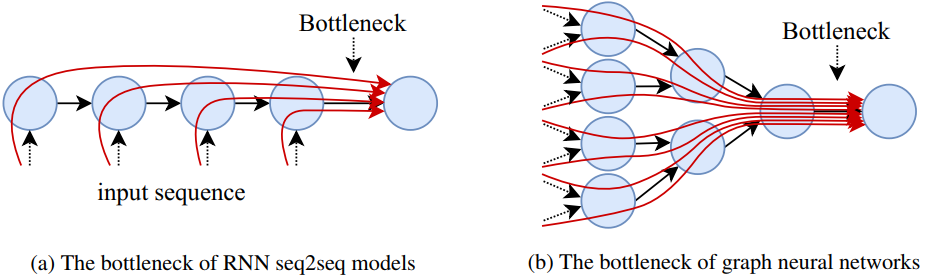
\includegraphics[width=.9\textwidth]{pics/bottleneck.png}
	\caption{The bottlenecks of Seq2seq and GNN models}
	\label{fig:bottleneck}
\end{figure}
作者将这个Bottleneck称为Over Suqashing,如Fig.\ref{fig:bottleneck}所示。什么是Over Squashing 呢?这就要从GNN的工作方式开始说起了。

GNN的工作方式是不断的将邻居结点的信息汇集(aggregate)起来,再进行后续的操作,通常一层汇聚的就是1-hop的邻居的信息,k层就可以汇聚到k-hop邻居的信息。随着层数的增加,一个结点的k-hop邻居的数量将会呈指数的形式增长,但是与前几层相比,更多的信息被压缩到了一个定长的向量中,这就是 over squashing。

在一些graph的任务中,不仅需要依靠局部的信息,如1-hop或者比较近的邻居的信息,同时还需要远距离的结点的信息。作者对任务所需要的邻居结点的距离定义为\textit{problem radius}。目前大部分使用的GNN都是比较浅层的,比如GCN的开山之作中就只有两层。作者在实验中还发现GCN、GIN比GAT等一些GNN模型更容易出现这个问题,显然,注意力机制在这里起了作用。

over squashing是指随着层数增加,指数速度增加的邻居的信息被过度压缩进了一个定长向量中,还有一个问题就是,对于最短路径大于GNN层数的情况,这个时候远距离的结点信息就不能传过来了,作者将其定义为under reaching。

作者在实验中发现,当\textit{problem radius}越大,则结点表征就需要更大的维度。

\paragraph{总结}

\begin{itemize}

	\item 将详细地研究了GNN中的远距离结点的信息的传播问题
	\item 之前的一些工作与这个有关,如\cite{li2019deepgcns}
	\item 有哪些较好地方法可以解决over squashing问题呢?
	\item 对于远距离结点地信息传播问题,能否通过在汇聚邻居信息时,随机采样较远的结点,作为远距离结点信息地补充
	\item 有哪些任务是需要远距离结点信息的呢?
	\item 能否用Transformer来作为GCN中的aggregate操作?

\end{itemize}

